%!TEX root = ../rules-working.tex
%LTeX: enabled=false

\addedin{1B}{1B-figures}{

\begin{onecolumnfigure}

\begin{fitheight}{3.2\standardhexwidth}
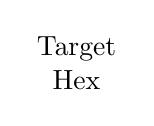
\begin{tikzpicture}
    \setfiguresize{-2.5}{-1.6}{+2.5}{+1.6}
    \drawhex{0}{0}  
    \drawhex{0}{+1}  
    \drawhex{0}{-1}  
    \drawhex{+1}{+0.5}  
    \drawhex{+1}{-0.5}  
    \drawhex{-1}{+0.5}  
    \drawhex{-1}{-0.5}  
    \drawhex[ultra thick,black]{0}{0}
    \node at (0,0) [align=center] {Target\\Hex};
\end{tikzpicture}
\end{fitheight}

\figurecaption{figure:blast-zone}{Blast and Fragmentation Danger Zone.}

\end{onecolumnfigure}
}
